\documentclass[11pt]{article}

\usepackage{float}
\usepackage{hyperref}
\usepackage{fullpage}
\usepackage{verbatim}
\usepackage{moreverb}
\usepackage{graphicx}
\usepackage{minted}
\let\verbatiminput=\verbatimtabinput
\def\verbatimtabsize{4\relax}

\begin{document}
\title{EECS 151/251A FPGA Lab\\
Lab 3: Useful Digital Circuits for Basic Signal Processing, Finite State Machines, Synchronous RAMS, and Synchronous Resets}

\author{Prof. Borivoje Nikolic \\
TA: Vighnesh Iyer \\Department of Electrical Engineering and Computer Sciences\\
College of Engineering, University of California, Berkeley}
\date{}
\maketitle

\section{Before You Start This Lab}

Before you proceed with the contents of this lab, we suggest that you look through three documents that will help you better understand some concepts we will be covering.

\begin{enumerate}
	\item \textbf{labs\_fa16/docs/Verilog/verilog\_fsm.pdf} - Goes over concepts of FSM in Verilog. Provides an example of  implementing FSM's in Verilog and pitfalls to watch out for.
	
	\item \url{http://www.labbookpages.co.uk/electronics/debounce.html} - Read "What is Switch Bounce" section to get idea of why we need a debouncer circuit. Read the "Digital Switch Debouncing" section to get a general overview of the circuit, its parts, and their purpose. You may want to pay attention to the purpose of the synchronizer as meta-stability is something you will go over in class. 
	
	\item \url{http://www.xilinx.com/products/boards/s3estarter/files/s3esk_rotary_encoder_interface.pdf} - Read page 5 (Rotary Encoder and Signals) to get an idea of how the encoder works and the signal it generates. You can read the next few pages to get a better idea of how to use the signals. 

\end{enumerate}

In the first couple sections of this lab, we will be revisiting the circuit you did in lab 2 and reconfirming functionality with actual music generated by the updated scripts. Then we will be going over some new circuits that you will be using in future assignments.

\subsection{Helpful Hint: Synthesis Warnings and Errors}
At various times in this lab, things will just not work on the FPGA or in simulation. To help with debugging, you can run \verb|make synth| in the \verb|lab2/| folder. This will just run \verb|xst| which will only take a few seconds. Then you should run \verb|make report|. In the window that opened, click on \verb|Synthesis Messages| on the left under \verb|Errors and Warnings|. Any synthesis warnings you see here are a possible alert to some issue in your circuit. If you don't understand a warning, ask a TA; it almost always reveals some issue in your RTL.

If your reports indicate there are no issues but you still have problems, please make sure that it is working in simulation. There is one case related to how memory is generated where you will likely get different results between simulation and actual FPGA behavior but we do not expect it to occur in this lab. This is an issue we will discuss in later in the lab. 

Also, you should try to keep the bit widths of the ROM and \verb|music_streamer| address consistent. You do not want to be changing them during the lab.

\section{Lab Overview}

In this lab, we will begin by taking your \verb|tone_generator| and \verb|music_streamer| design from Lab 2 and feeding it parts of real music. We will learn about circuits to take the signals generated by our buttons and rotary encoder and convert them into a digital signal we can use within our digital clock domain. You will be using the LED's to confirm they are working correctly. We will also be going over properly using synchronous resets to refresh the state of the circuits. 

\section{Tone\_generator With Music}

\subsection{Overview of Your Tone\_generator and Music\_streamer}

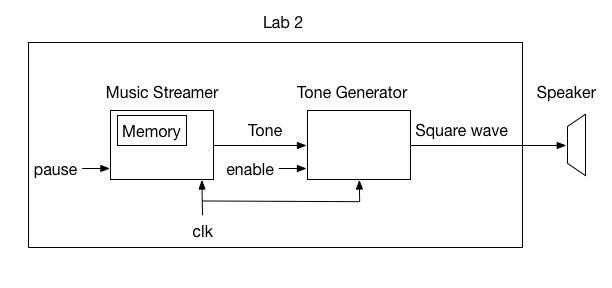
\includegraphics[width=\textwidth]{images/lab2_fig1.png}

We included this diagram so you can review the circuit you made in lab 2. There are two main modules that you created: \verb|tone_generator| and \verb|music_streamer|. 

Your \verb|tone_generator| should take an input signal representing the tone or frequency you want to play and output an oscillating signal that goes to the speaker. It has an enable signal that basically turns if off and on, and this enable signal should be hooked up to one of the DIP switches.  

Your \verb|music_streamer| is responsible for providing the input signal to your \verb|tone_generator| so it knows what frequency to play. Inside this generator is the memory (ROM for lab 2), that holds the frequencies you want to play. Your music generator will output one tone for a certain amount of time (1/5 of a second for lab 2) before updating its address to its memory. This new address should point to the next frequency you want to play. Your \verb|music_streamer| will keep incrementing its address until it reaches the end of the ROM in which case, it reset back to the first address, and plays your tones from the beginning again. 

We will be adding two new circuits to what we already have to give our music circuit more functionality.

\subsection{Playing Music}
Run \verb|git pull| in your git cloned \verb|labs_fa16| directory to fetch the latest skeleton files.

Begin by copying your \verb|tone_generator| and \verb|music_streamer| implementation into the \newline \verb|lab2/tone_generator.v| and \verb|lab2/music_streamer.v| files. Run 
\begin{minted}{verilog}
python musicXML_parser.py input_xml_file.xml output_text_file.txt
\end{minted}
This basically converts some sheet music (in the form of an XML file) into the text files you used in previous labs to generate the ROMs. Now run the same command from the previous lab
\begin{minted}{verilog}
python rom_generator.py src/rom.v output_text_file.txt 1024 24
\end{minted}

Keep in mind there are two new things you want to take into account. We've made the depth of the ROM 1024 entries now but the it is likely the piece of music you will be playing is not that long. The ROM module generated by the script should now have an extra output \verb




\section{Conclusion}

\end{document}